%%%% This Beamer example was created by LianTze Lim, April 2017.

%%%% This is a VERY simple and minimalistic beamer theme,
%%%% even reminiscent of marker pens on transparencies!
%%%% It mimics the look of the "seminar" package, which
%%%% can only be used with plain TeX.
%%%% There are also some comments and example to show how
%%%% to customise various elements, e.g. the font and colours.

\documentclass[12pt]{beamer}
%% If you'd like the default font size to be even larger, use 14pt or 17pt; these are supported by Beamer.

\usepackage[english]{babel}
\usepackage[utf8]{inputenc}
\usepackage[T1]{fontenc}
\usepackage{lmodern}

\usepackage{listings}

%%%%%%%%%%%%%%%%%%%%%%%%%%%%%%%%%%%%%%%%%
% These lines should usually go into a .sty file,
% but I'll leave them here so that it's easier to
% see how to customise a Beamer theme.
% Remember, the Beamer manual is your friend!!
% http://texdoc.net/pkg/beamer
%
%% So if your re-definitions have a @ somewhere, you
%% _MUST_ put a \makeatletter before these lines and then
%% \makeatother after them. This trick can only be done
%% in the preamble! BUT if you're doing these re-definitions
%% in a .sty file (so that you \usepackage it later), you
%% don't need the \makeatletter and \makeatother.
\makeatletter

%% Set the left and right margins
\setbeamersize{text margin left=1em,text margin right=1em}

%% FONTS
\setbeamerfont{title}{series=\bfseries,size=\LARGE}
\setbeamerfont{subtitle}{series=\bfseries,size=\Large}
\setbeamerfont{frametitle}{series=\bfseries,size=\small}
\setbeamerfont{block title}{series=\bfseries,size=\normalsize}
\setbeamerfont{footline}{size=\normalsize}

%% COLOURS
%% If you'd like everything to have the same colour
\usebeamercolor{structure}
\setbeamercolor{normal text}{fg=structure.fg}

%% Add a line after the frametitle
\addtobeamertemplate{frametitle}{}{\vspace*{-1ex}\rule{\textwidth}{1pt}}

%% Use circular discs as itemized list markers;
%% there's an existing option in Beamer for it so I'll use it
\setbeamertemplate{itemize items}[circle]

%% Remove default navigation symbols (We'll add the ones we need in the footline
\setbeamertemplate{navigation symbols}{}


%% And before the footline... actually we'd like to re-define
%% the footline
\setbeamertemplate{footline}{%
   %% Beamer headlines and footlines are always full-paperwidth, so if you want the horizontal line to
   %% not span it entirely you'll need to do a bit of arithmetic
   \centering
   \begin{minipage}{\dimexpr\paperwidth-\beamer@leftmargin-\beamer@rightmargin\relax}
   \centering
   \rule{\linewidth}{1pt}\vskip2pt
   \usebeamerfont{footline}%
   \usebeamercolor{footline}%
   %% The frame number smack in the middle
   \hfill\insertpagenumber/\inserttotalframenumber
   \hfill%
   %% ONLY the navigation symbols we want at the far right.
   %% We use an \llap so that it takes up zero width, and doesn't throw the page number off-centre!
   \llap{\insertframenavigationsymbol\insertbackfindforwardnavigationsymbol}\par
   \end{minipage}\vskip2pt
}

\makeatother
%%%% END STYLE CUSTOMISATION %%%%%%%%%%%%

\title{Zmiana karty do głosowania a odsetek głosów
nieważnych w wyborach do rad gmin}
\subtitle{Eksperyment naturalny}
\author{Michał Pierzgalski, Maciej Górecki, Paweł Stępień}
\institute{Uniwersytet Łódzki, Uniwersytet Warszawski}
\date{Wrzesień 2018}

\begin{document}

\begin{frame}
  \titlepage
\end{frame}

% Uncomment these lines for an automatically generated outline.
%\begin{frame}{Outline}
%  \tableofcontents
%\end{frame}

\section{Introduction}


\begin{frame}{Plan wystąpienia}
    
\begin{enumerate}
\item O metodzie \textit{generalized synthetic control} - metoda porównywania grupy eksperymentalnej i kontrolnej w badaniach \textit{quasi}-eksperymentalnych;
\item Przykłady zastosowania metody:
\begin{itemize}
\item efekt kwot wyborczych dla kobiet (przypadek systemów OLPR - np. wybory do Sejmu RP),
\item efekt ``książeczki''; \textit{redesign} karty do głosowania a odsetek głosów nieważnych w wyborach do rad w miastach na prawach powiatu 2014.
\end{itemize}
\end{enumerate}

\end{frame}

\section{Metoda}


\begin{frame}{Wprowadzenie}

\begin{block}{Metoda}
\begin{itemize}
\item \textbf{Uogólniona metoda syntetycznej grupy/jednostki kontrolnej} (\textit{generalized sytnthetic control}, Yiqing Xu (2017)) - nowoczesna metoda porównywania \textbf{grupy kontrolnej} i \textbf{grupy eksperymentalnej} (badania \textit{quasi}-eksperymentalne)
\end{itemize}
\end{block}

\end{frame}


\begin{frame}{Metoda}

\begin{block}{\textit{Differences-in-differences}}
W analizie porównawczej grupy \textbf{kontrolnej} i \textbf{eksperymentalnej} zwykle korzysta się z tzw. metody \textit{differences-in-differences} (DID)
\end{block}

\end{frame}

\begin{frame}{Metoda}

\begin{figure}
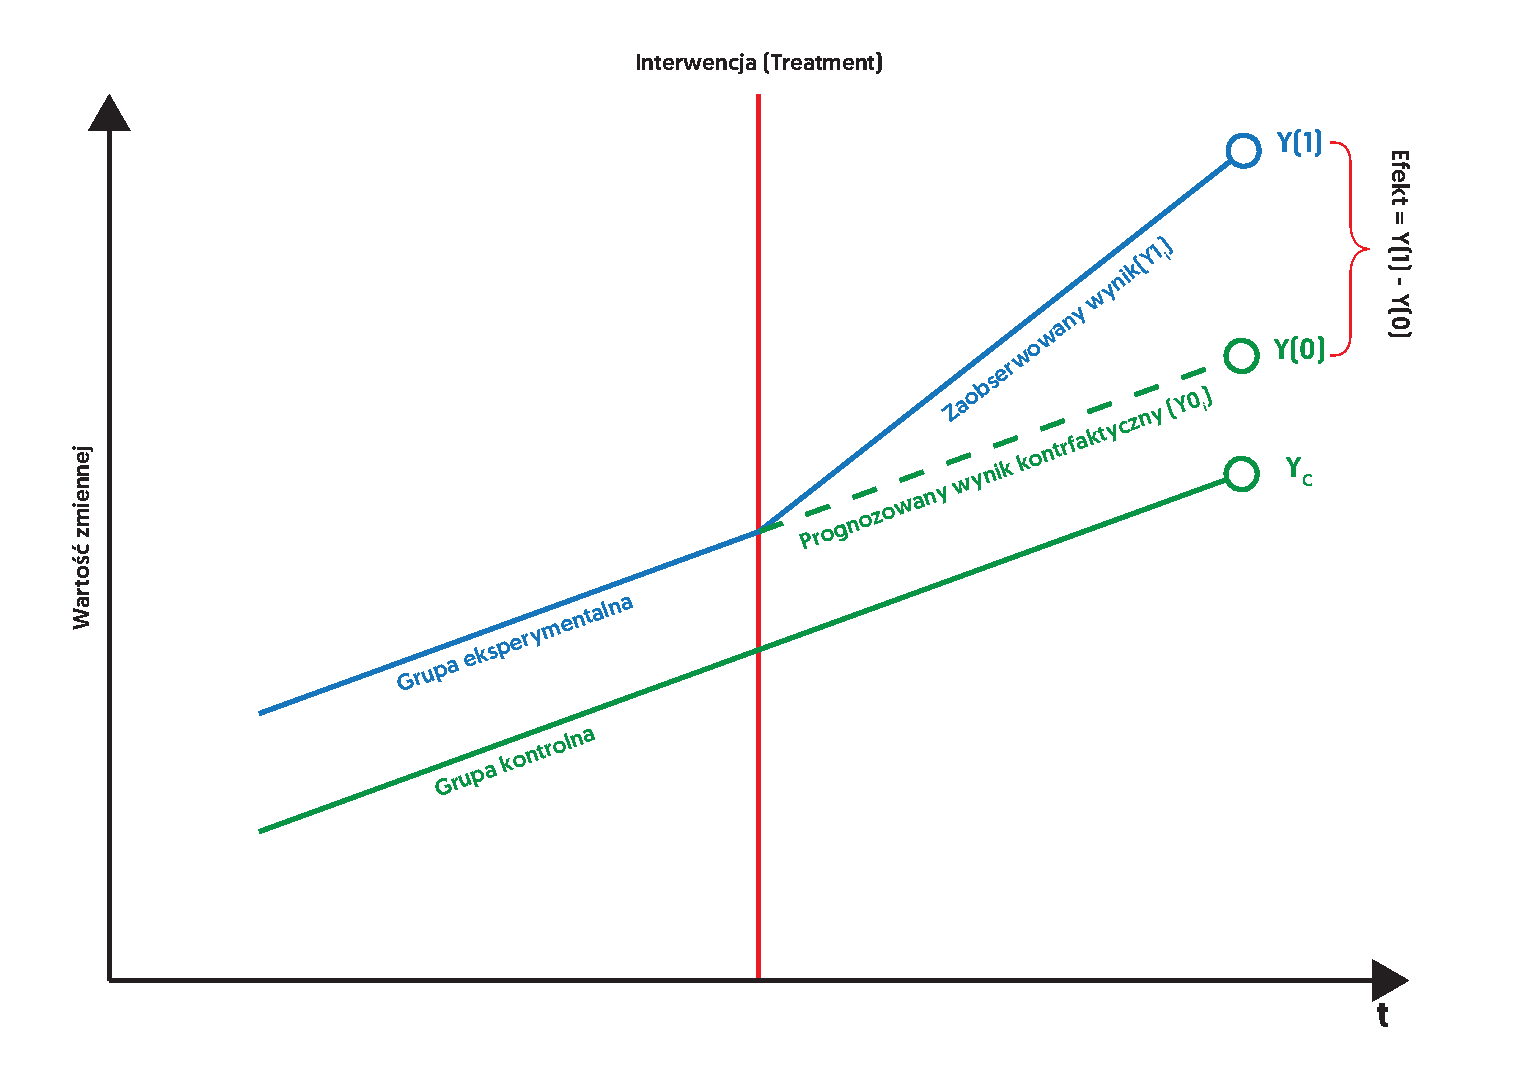
\includegraphics[scale=0.35]{did.pdf}
\caption{\label{fig:did}\textit{Treatment effect} w eksperymentach naturalnych}
\end{figure}

\end{frame}


\begin{frame}{Metoda}

\begin{block}{Postać funkcyjna modelu regresji dla metody DID}
$$ y_{it} = \alpha + \gamma Treat_i + \eta Post_t + \delta_r (Treat_i \times Post_t) + x_{it}^{'}\beta + e_{it} $$

\scriptsize

\textbf{gdzie}: $Treat_i$ - binarny wskaźnik grupy kontrolnej; $Post_t$ - binarny wskaźnik obserwacji po interwencji; $x_{it}$ to $(k \times 1)$ wektor obserwacji na predyktorach; $\beta$ jest $(k \times 1)$ wektorem nieznanych wartości parametrów; $\delta_r$ jest \textbf{estymatorem efektu ``differences-in-differences''}; $e_{it}$ oznacza błąd standardowy dla jednostki $i$ w czasie $t$.
\end{block}

\end{frame}

\begin{frame}{Podstawowe ograniczenia metody DID}
    
\begin{block}{\textit{Parallel trends} i \textit{selection bias}}
\begin{itemize}
\item Założenie równoległości trendów (grupa eksperymentalna $||$ grupa kontrolna) - \textit{parallel trends assumption};
\item \textit{selection bias} - problem podobieństwa jednostek tworzących grupy eksperymentalną i kontrolną.
\end{itemize}
\end{block}
    
\end{frame}
   
\begin{frame}{Generalized synthetic control}

\begin{block}{Remedium:}
\textit{Uogólniona metoda syntetycznej jednostki kontrolnej} (\textbf{GSC}) zaproponowana przez Xu (2017) na łamach "Political Analysis".
\end{block}

Pierwotna wersja metody została zaproponowana przez Alberto \textbf{Abadie}, A. \textbf{Diamond} i J. \textbf{Haimueller} w \textit{Journal of the American Statistical Association}.

\begin{itemize}
\item Bardzo obiecująca metoda badawcza, ale skomplikowana matematycznie i jeszcze niewystarczająco przetestowana w praktyce badawczej;
\item Metoda z dużym potencjałem zastosowania m.in. w obszarze \textit{comparative politics}.
\end{itemize}

\end{frame}


\begin{frame}{Metoda}

\begin{block}{Dlaczego GSC?}
\begin{itemize}
\item Jest zaawansowanym narzędziem umożliwiającym stworzenie ``syntetycznej jednostki kontrolnej'', która dobrze odzwierciedla cechy jednostek w grupie eksperymentalnej;
\item Nie wymaga przyjęcia ``parallel trends assumption''.
\end{itemize}
\end{block}

\end{frame}


\begin{frame}{Metoda}

\textbf{Syntetyczna jednostka kontrolna} w metodzie GSC jest tworzona:
\begin{enumerate}
\item z użyciem modelu \textit{interactive fixed effect} (\textbf{IFE}), albo
\item stosując tzw. metodę uzupełniania macierzy danych (\textit{matrix completion method} (\textbf{MC})).
\end{enumerate}

\end{frame}

\begin{frame}{Metoda}

\begin{block}{Postać funkcyjna GSC (estymator IFE)}
$$ y_{it} = \delta_{it} D_{it} + x_{it}^{'}\beta + \lambda_i^{'} f_t + e_{it} $$

\scriptsize

\textbf{gdzie}: $D_{it}$ zero-jedynkowy wskaźnik interwencji eksperymentalnej; $\delta_{it}$ estymator efektu interwencji; $x_{it}$ - $(k \times 1)$ wektor obserwacji na predyktorach; $\beta$ - $(k \times 1)$ wektor wartości nieznanych parametrów; $f_t$ - $(r \times 1)$ wektor nieobserwowalnych czynników (latent factors); $\lambda_i$ - $(r \times 1)$ wektor nieznanych ładunków czynnikowych (factor loadings); $e_{it}$ błąd standardowy dla jednostki $i$ w czasie $t$.
\end{block}

\end{frame}

\begin{frame}{Metoda}

\begin{block}{Implementacja metody GSC}
Analizę z użyciem GSC można obecnie wykonać stosując pakiet funkcji \textit{gsynth} języka programowania R - autorem pakietu są Y. Xu (twórca metody) i L. Liu.
\end{block}

Pakiet \textit{gsynth}:
\begin{itemize}
\item umożliwia wizualizację modelu (dość łatwa interpretacja wyniku badania),
\item dostarcza narzędzi pozwalających ocenić ``jakość'' utworzonej syntetycznej jednostki kontrolnej,
\item pozwala ocenić czy ATT (przeciętny efekt interwencji) jest istotny statystycznie (\textit{p-value}).
\end{itemize}

\end{frame}


\begin{frame}{Metoda}

\begin{figure}
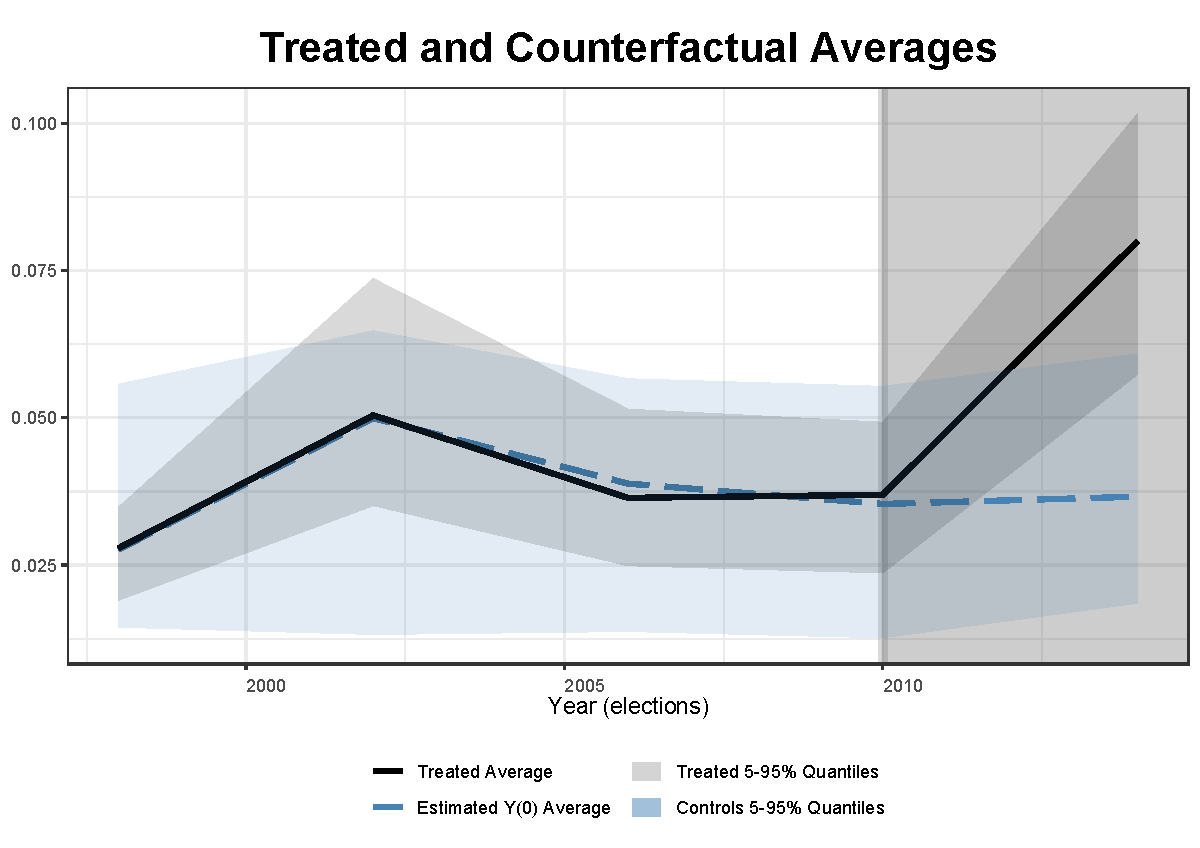
\includegraphics[scale=0.42]{ife_no_pred_2_factors_sample_0_2_band}
\caption{\label{fig:did}Przykład wizualizacji wyniku badania w metodzie GSC}
\end{figure}

\end{frame}


\begin{frame}{Metoda}

\begin{block}{Niektóre trudności związane z aplikacją GSC}
\begin{itemize}
\item Wspomniany wyżej poziom formalnego skomplikowania modelu;
\item Wymaga przynajmniej 3-4 (najlepiej kilkunastu lub więcej) okresów obserwacyjnych przed ``interwencją eksperymentalną'';
\item W przypadku dużej próby, estymacja parametrów modelu może trwać długo (potrzebny szybki komputer);
\item Metoda jest w trakcie testowania, jest nadal ulepszana/modyfikowana.
\end{itemize}
\end{block}

\end{frame}

\section{Wyniki}

\begin{frame}{Zastosowanie metody - efekt "książeczki"}

\begin{block}{O badaniu}
\begin{itemize}
\item Projekt karty do głosowania może wpływać na wyniki wyborów. W szczególności, wadliwy ``design'' karty może spowodować zwiększenie odsetka głosów nieważnych.
\item Przedstawiamy wstępne wyniki \textit{quasi}-eksperymentalnego badania wpływu zastosowania karty do głosowania w formie tzw. książeczki w wyborach (2014) do \textbf{rad w miastach na prawach powiatu} (grupa eksperymentalna).
\end{itemize}
\end{block}

\end{frame}

\begin{frame}{Karta wyborcza a głosy nieważne - wstępne wyniki badania}
    
\begin{block}{Dane}
\begin{itemize}
\item W badaniu wykorzystano oficjalne dane \textbf{PKW} dotyczące \textbf{głosów nieważnych w okręgach}, dla wyborów do rad gmin/miast, w okresie \textbf{1998-2014};
\item W eksperymencie użyto \textbf{mediany} odsetka głosów nieważnych dla okręgów w gminie (miasta na prawach powiatu, gminy miejsko-wiejskie i gminy wiejskie);
\item Zmienne \textbf{kontrolne}: stosunek liczby kandydatów w gminie do liczby mandatów \textit{oraz} typ formuły wyborczej.
\end{itemize}
\end{block}
    
\end{frame}

\begin{frame}{Wstępne wyniki badania - wizualizacja tzw. efektu "książeczki" w 2014 (1)}
    
\begin{figure}
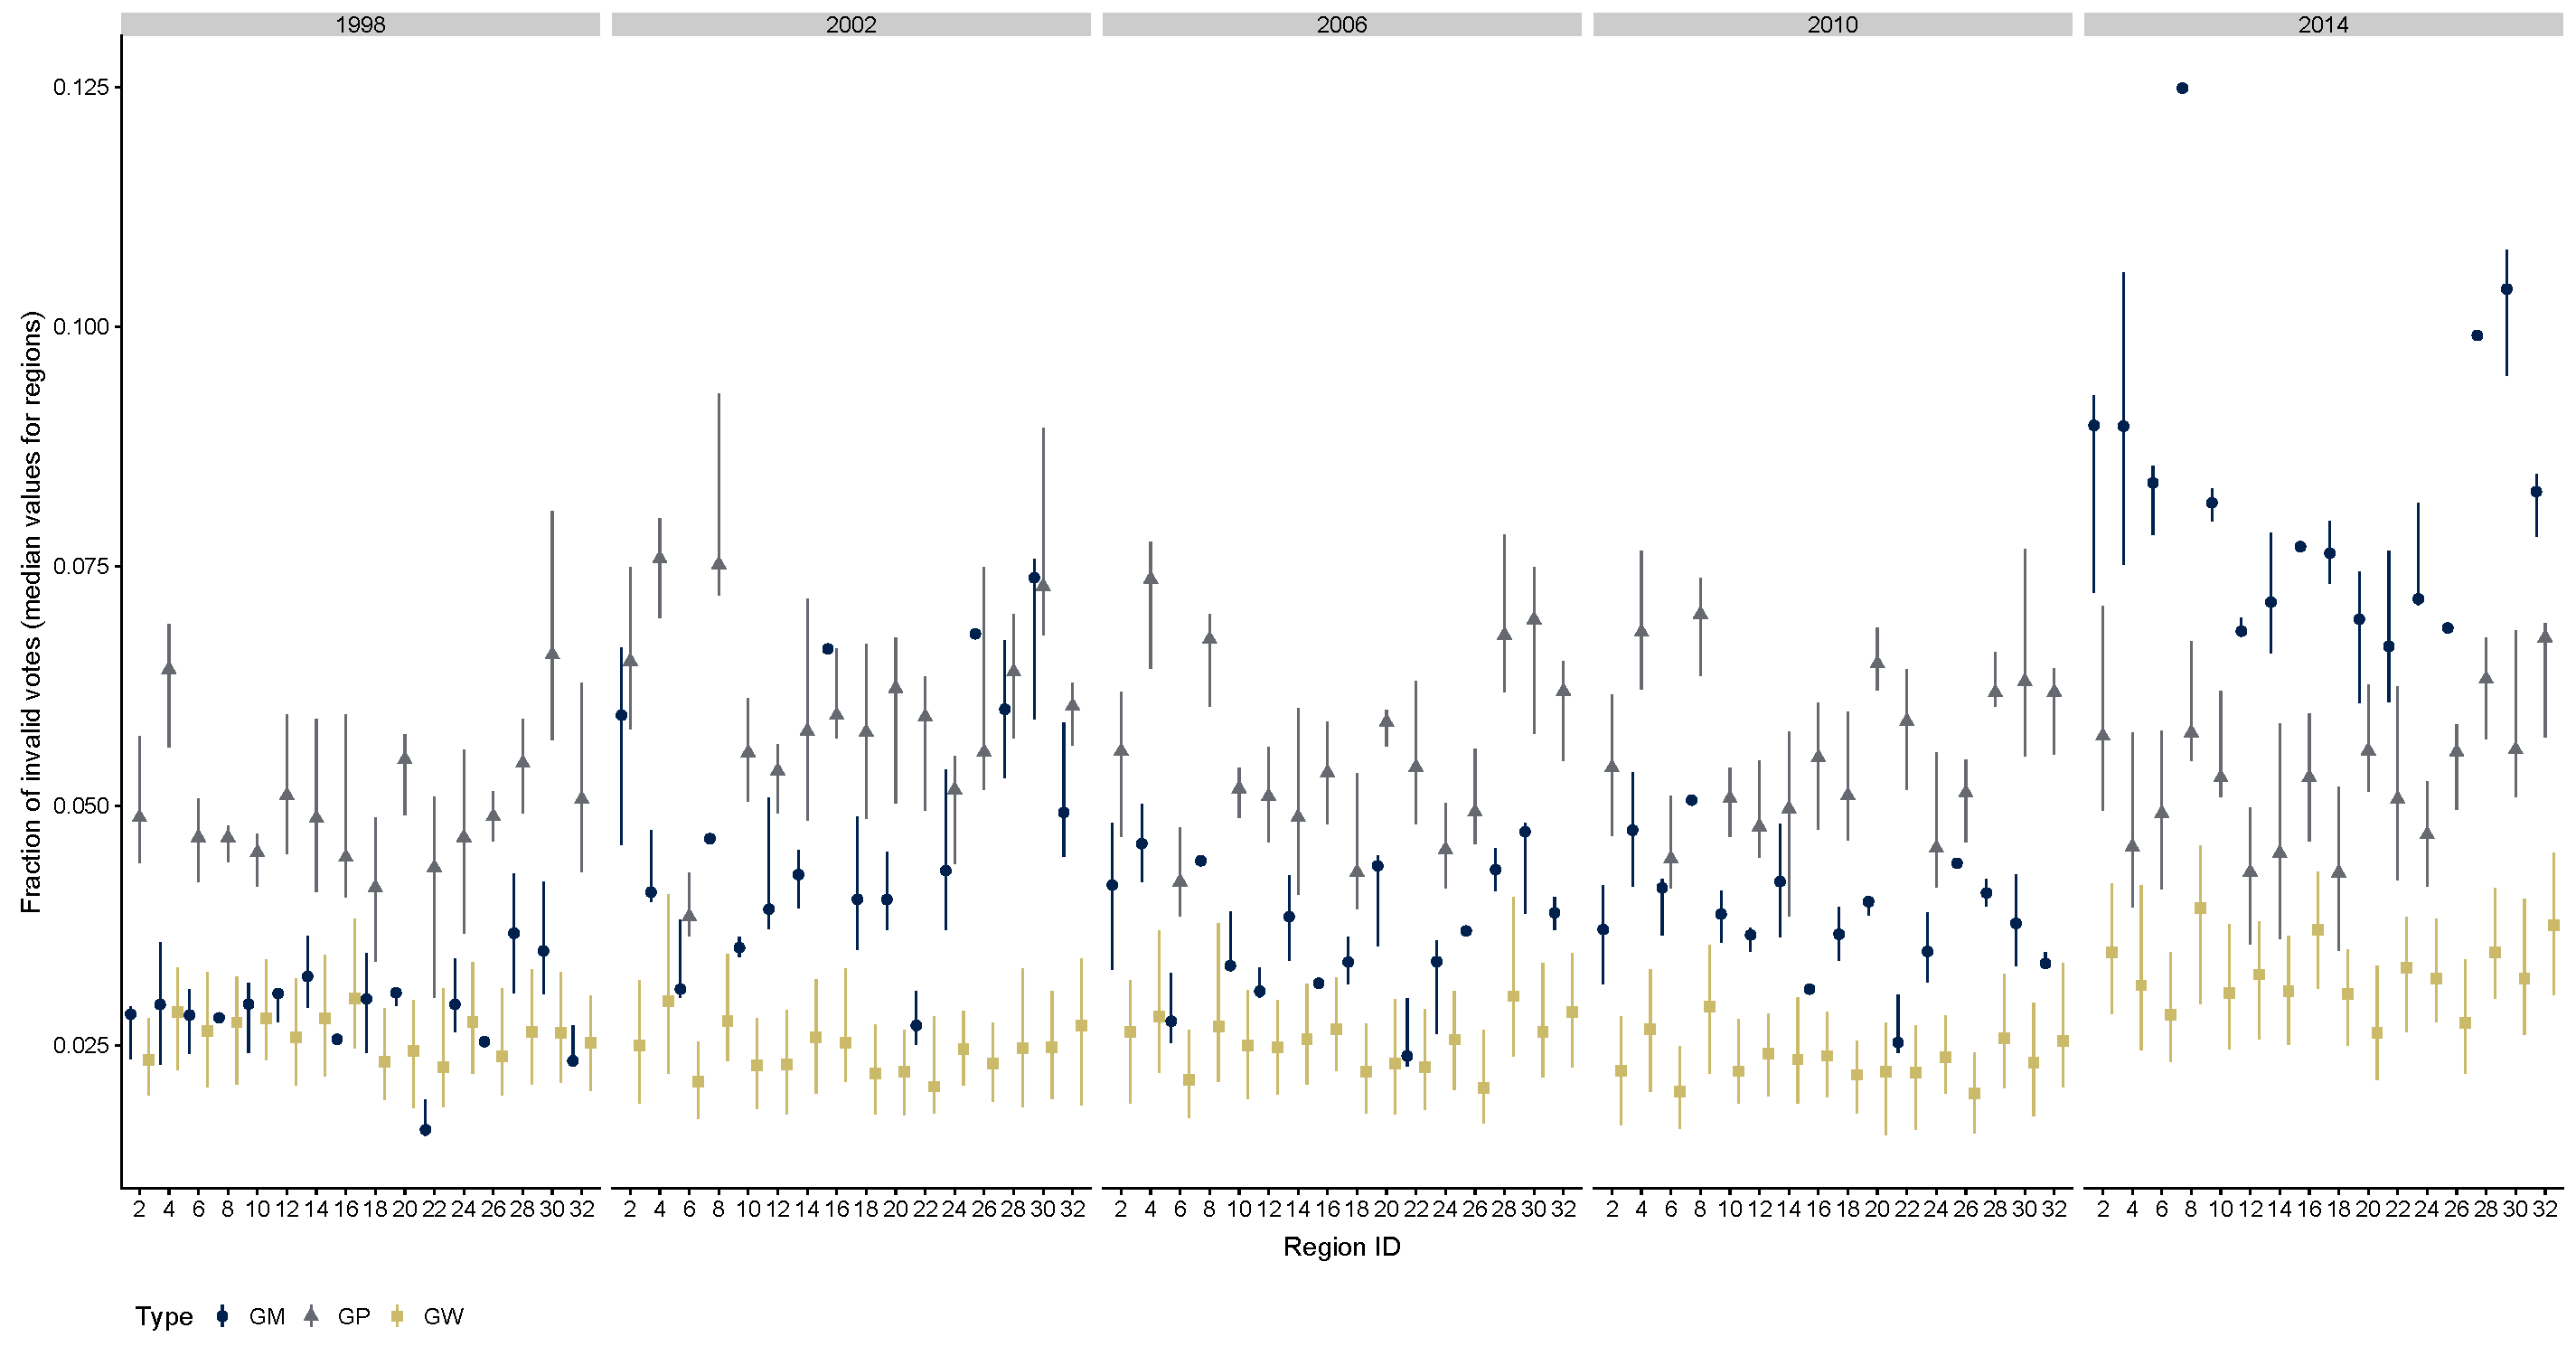
\includegraphics[scale=0.22]{inv_medians.pdf}
\caption{\label{fig:did}Kwartyl 2 (mediana) oraz 1 i 3 (poziom regionu) dla gminnych median ułamków głosów nieważnych w okręgach wyborczych}
\end{figure}
    
\end{frame}


\begin{frame}{Wstępne wyniki badania - wizualizacja tzw. efektu "książeczki" w 2014 (1)}
    
\begin{figure}
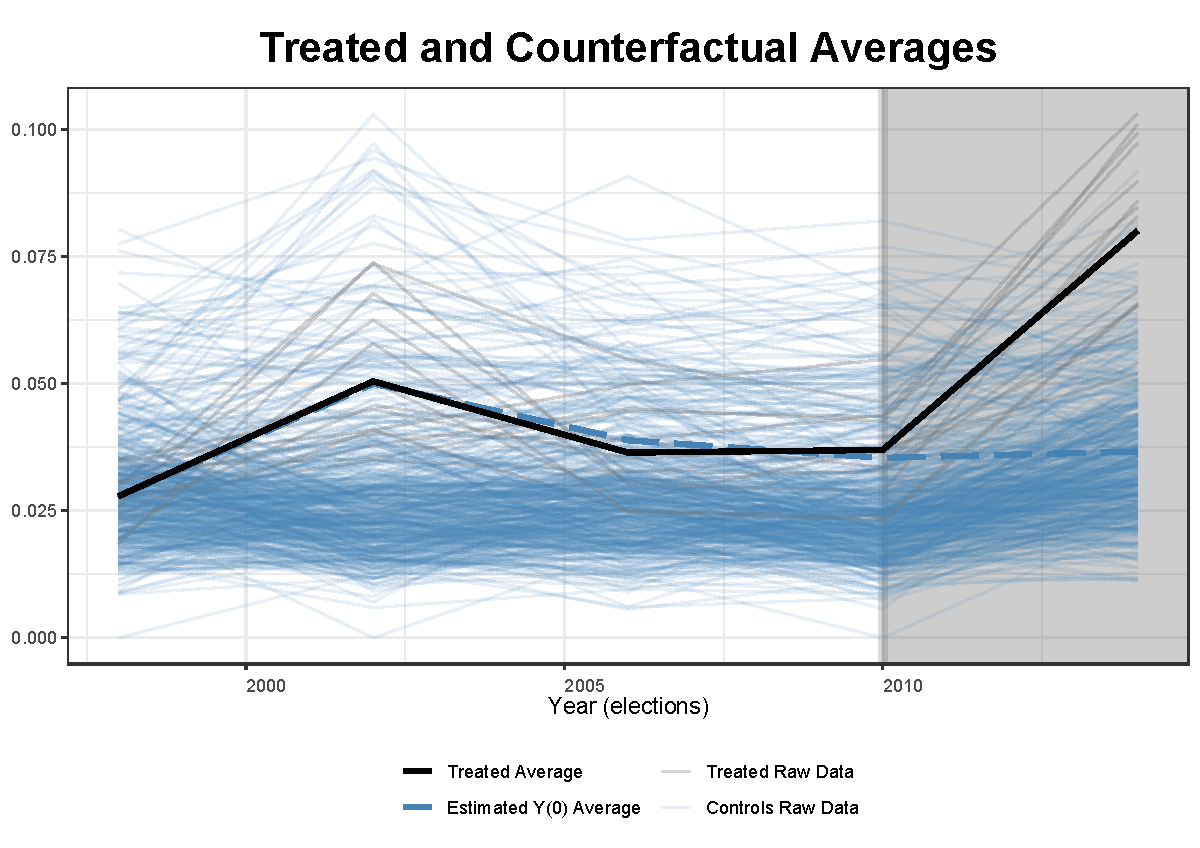
\includegraphics[scale=0.43]{ife_no_pred_2_factors_sample_0_2_raw.pdf}
\caption{\label{fig:did}Przykład wizualizacji wyniku badania w metodzie GSC}
\end{figure}
    
\end{frame}

\begin{frame}{Wstępne wyniki badania - wizualizacja tzw. efektu "książeczki" w 2014 (2)}
    
\begin{figure}
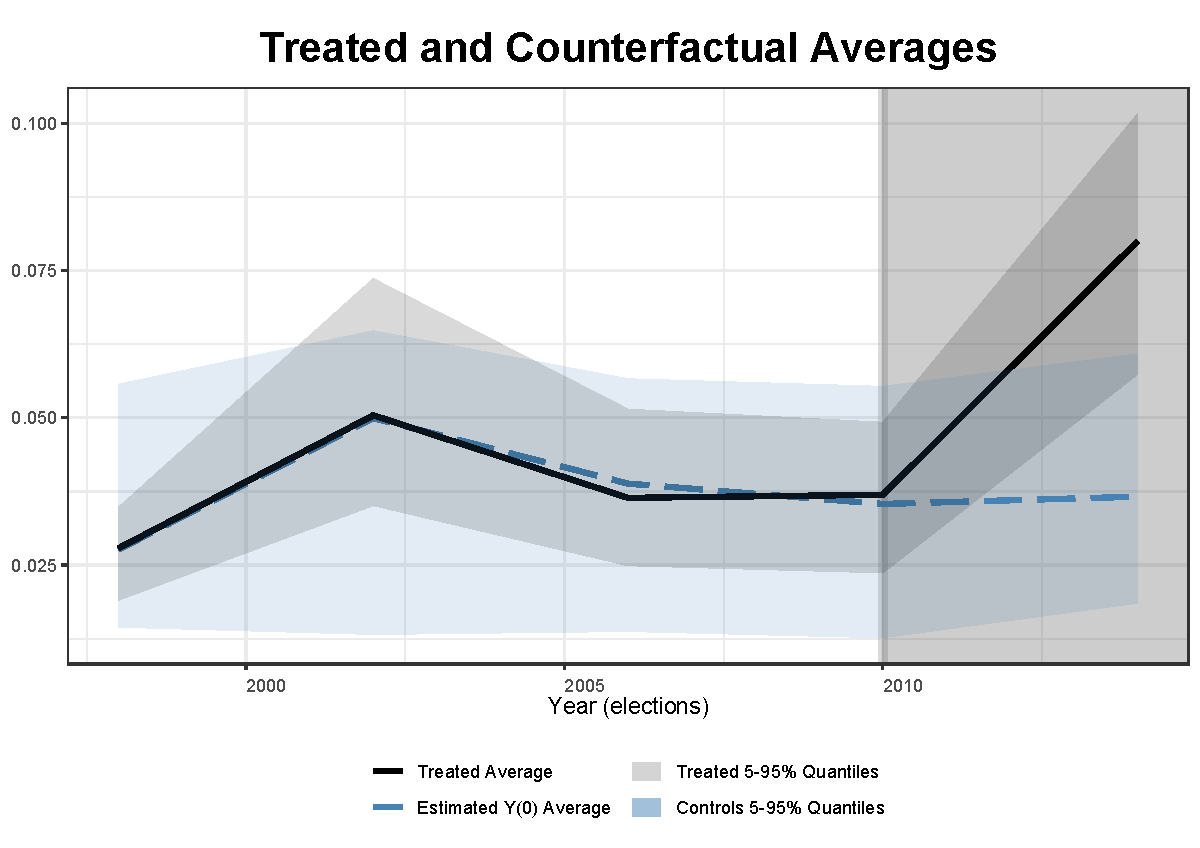
\includegraphics[scale=0.43]{ife_no_pred_2_factors_sample_0_2_band}
\caption{\label{fig:did}Przykład wizualizacji wyniku badania w metodzie GSC}
\end{figure}
    
\end{frame}

\begin{frame}{Wstępne wyniki badania - wizualizacja tzw. efektu "książeczki" w 2014 (3)}
    
\begin{figure}
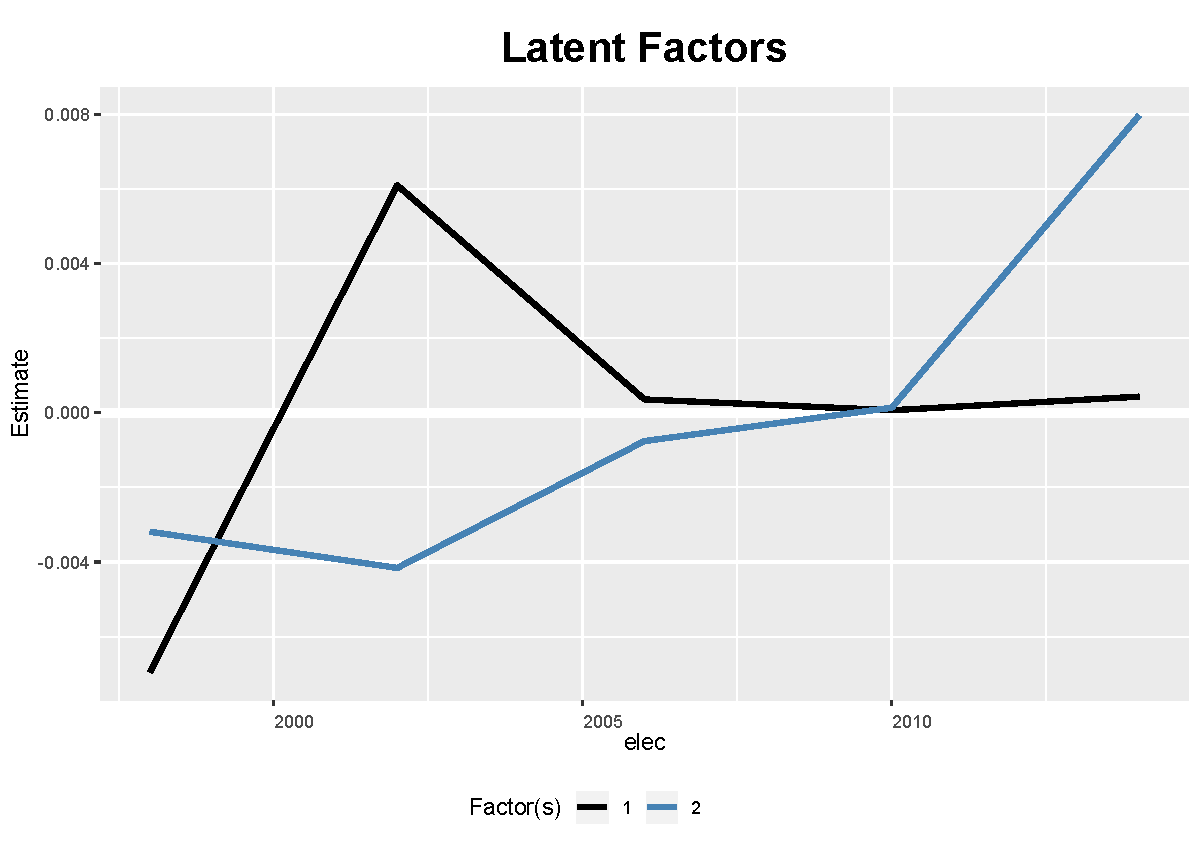
\includegraphics[scale=0.43]{ife_no_pred_2_factors_sample_0_2_factors.pdf}
\caption{\label{fig:did}Wykres dynamiki czynników}
\end{figure}
    
\end{frame}

\begin{frame}[fragile]{Przykładowa specyfikacja modelu dla losowej próby 499 gmin}

\scriptsize

\begin{lstlisting}{language=R}
Average Treatment Effect on the Treated:
 ATT.avg     S.E. CI.lower CI.upper p.value
  0.0434 0.007036  0.02955  0.05597       0

   ~ by Period (including Pre-treatment Periods):
         ATT      S.E.     CI.lower   CI.upper p.value n.Treated
1  0.0002292 0.0001345  0.000001179 0.00054935    0.05         0
2  0.0004626 0.0002246  0.000140676 0.00116601    0.01         0
3 -0.0024217 0.0012514 -0.004905261 0.00001382    0.06         0
4  0.0015666 0.0011014 -0.001058276 0.00328988    0.21         0
5  0.0433983 0.0070361  0.029551162 0.05596624    0.00        14
\end{lstlisting}

\end{frame}

\begin{frame}{Efekt kwot wyborczych}
\[ \rightarrow \]
\end{frame}

\end{document}
